% Options for packages loaded elsewhere
\PassOptionsToPackage{unicode}{hyperref}
\PassOptionsToPackage{hyphens}{url}
\PassOptionsToPackage{dvipsnames,svgnames,x11names}{xcolor}
%
\documentclass[
  letterpaper,
  DIV=11,
  numbers=noendperiod]{scrreprt}

\usepackage{amsmath,amssymb}
\usepackage{iftex}
\ifPDFTeX
  \usepackage[T1]{fontenc}
  \usepackage[utf8]{inputenc}
  \usepackage{textcomp} % provide euro and other symbols
\else % if luatex or xetex
  \usepackage{unicode-math}
  \defaultfontfeatures{Scale=MatchLowercase}
  \defaultfontfeatures[\rmfamily]{Ligatures=TeX,Scale=1}
\fi
\usepackage{lmodern}
\ifPDFTeX\else  
    % xetex/luatex font selection
\fi
% Use upquote if available, for straight quotes in verbatim environments
\IfFileExists{upquote.sty}{\usepackage{upquote}}{}
\IfFileExists{microtype.sty}{% use microtype if available
  \usepackage[]{microtype}
  \UseMicrotypeSet[protrusion]{basicmath} % disable protrusion for tt fonts
}{}
\makeatletter
\@ifundefined{KOMAClassName}{% if non-KOMA class
  \IfFileExists{parskip.sty}{%
    \usepackage{parskip}
  }{% else
    \setlength{\parindent}{0pt}
    \setlength{\parskip}{6pt plus 2pt minus 1pt}}
}{% if KOMA class
  \KOMAoptions{parskip=half}}
\makeatother
\usepackage{xcolor}
\setlength{\emergencystretch}{3em} % prevent overfull lines
\setcounter{secnumdepth}{5}
% Make \paragraph and \subparagraph free-standing
\ifx\paragraph\undefined\else
  \let\oldparagraph\paragraph
  \renewcommand{\paragraph}[1]{\oldparagraph{#1}\mbox{}}
\fi
\ifx\subparagraph\undefined\else
  \let\oldsubparagraph\subparagraph
  \renewcommand{\subparagraph}[1]{\oldsubparagraph{#1}\mbox{}}
\fi


\providecommand{\tightlist}{%
  \setlength{\itemsep}{0pt}\setlength{\parskip}{0pt}}\usepackage{longtable,booktabs,array}
\usepackage{calc} % for calculating minipage widths
% Correct order of tables after \paragraph or \subparagraph
\usepackage{etoolbox}
\makeatletter
\patchcmd\longtable{\par}{\if@noskipsec\mbox{}\fi\par}{}{}
\makeatother
% Allow footnotes in longtable head/foot
\IfFileExists{footnotehyper.sty}{\usepackage{footnotehyper}}{\usepackage{footnote}}
\makesavenoteenv{longtable}
\usepackage{graphicx}
\makeatletter
\def\maxwidth{\ifdim\Gin@nat@width>\linewidth\linewidth\else\Gin@nat@width\fi}
\def\maxheight{\ifdim\Gin@nat@height>\textheight\textheight\else\Gin@nat@height\fi}
\makeatother
% Scale images if necessary, so that they will not overflow the page
% margins by default, and it is still possible to overwrite the defaults
% using explicit options in \includegraphics[width, height, ...]{}
\setkeys{Gin}{width=\maxwidth,height=\maxheight,keepaspectratio}
% Set default figure placement to htbp
\makeatletter
\def\fps@figure{htbp}
\makeatother

\KOMAoption{captions}{tableheading}
\makeatletter
\@ifpackageloaded{bookmark}{}{\usepackage{bookmark}}
\makeatother
\makeatletter
\@ifpackageloaded{caption}{}{\usepackage{caption}}
\AtBeginDocument{%
\ifdefined\contentsname
  \renewcommand*\contentsname{Table of contents}
\else
  \newcommand\contentsname{Table of contents}
\fi
\ifdefined\listfigurename
  \renewcommand*\listfigurename{List of Figures}
\else
  \newcommand\listfigurename{List of Figures}
\fi
\ifdefined\listtablename
  \renewcommand*\listtablename{List of Tables}
\else
  \newcommand\listtablename{List of Tables}
\fi
\ifdefined\figurename
  \renewcommand*\figurename{Figure}
\else
  \newcommand\figurename{Figure}
\fi
\ifdefined\tablename
  \renewcommand*\tablename{Table}
\else
  \newcommand\tablename{Table}
\fi
}
\@ifpackageloaded{float}{}{\usepackage{float}}
\floatstyle{ruled}
\@ifundefined{c@chapter}{\newfloat{codelisting}{h}{lop}}{\newfloat{codelisting}{h}{lop}[chapter]}
\floatname{codelisting}{Listing}
\newcommand*\listoflistings{\listof{codelisting}{List of Listings}}
\makeatother
\makeatletter
\makeatother
\makeatletter
\@ifpackageloaded{caption}{}{\usepackage{caption}}
\@ifpackageloaded{subcaption}{}{\usepackage{subcaption}}
\makeatother
\ifLuaTeX
  \usepackage{selnolig}  % disable illegal ligatures
\fi
\usepackage{bookmark}

\IfFileExists{xurl.sty}{\usepackage{xurl}}{} % add URL line breaks if available
\urlstyle{same} % disable monospaced font for URLs
\hypersetup{
  pdftitle={Lecture fire simulation},
  pdfauthor={Lukas Arnold},
  colorlinks=true,
  linkcolor={blue},
  filecolor={Maroon},
  citecolor={Blue},
  urlcolor={Blue},
  pdfcreator={LaTeX via pandoc}}

\title{Lecture fire simulation}
\author{Lukas Arnold}
\date{2024-04-23}

\begin{document}
\maketitle

\renewcommand*\contentsname{Table of contents}
{
\hypersetup{linkcolor=}
\setcounter{tocdepth}{2}
\tableofcontents
}
\bookmarksetup{startatroot}

\chapter*{Overview}\label{overview}
\addcontentsline{toc}{chapter}{Overview}

\markboth{Overview}{Overview}

\section*{General Information}\label{general-information}
\addcontentsline{toc}{section}{General Information}

\markright{General Information}

The lecture \emph{Fire Simulations} at the University of Wuppertal is
organised by the chair of
\href{https://cce.uni-wuppertal.de/}{Computational Civil Engineering
(CCE)}. The 2019 founded chair is mainly concerned with the research and
development of new computer-based models. The focus of the application
is the numerical simulation of fire and smoke propagation in buildings.

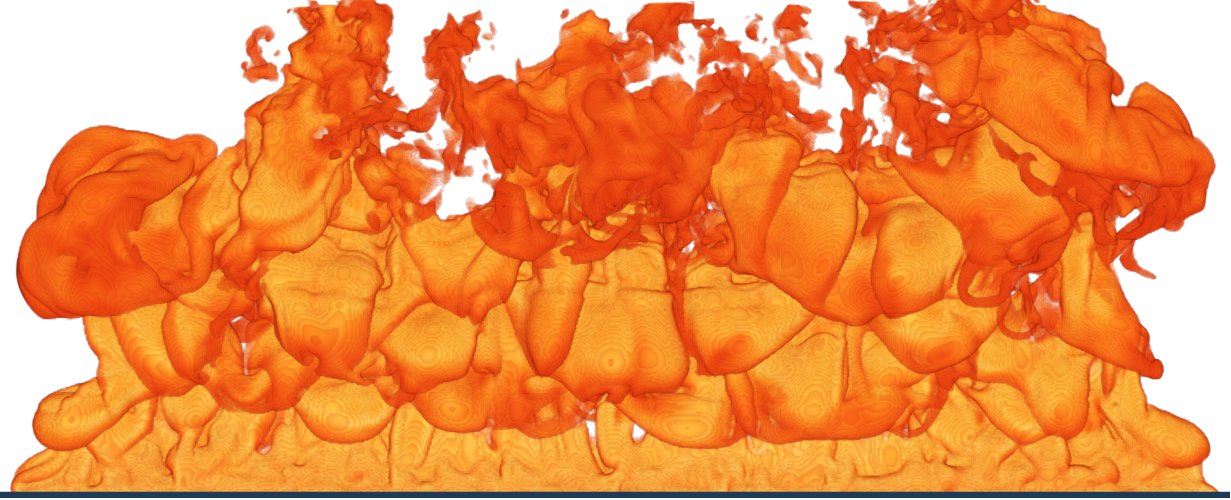
\includegraphics{./content/00_overview/figs/fire_banner.png}

This is the first year that we offer this script. The motivation to
create this script is on the one hand to give the participants of the
lecture a possibility to read the contents. And on the other hand, to
make this content freely available to external or former participants.

However, this script is very short and will remain so. Much of the
content is already available in greater depth, so that reference is made
to the relevant passages - instead of simply copying them.

As the script is under development, we welcome constructive suggestions
and your feedback. This way you can support our whole fire science
community.

\textbf{For the University of Wuppertal students: All organisational
information on the procedure can be found on the
\href{https://cce.uni-wuppertal.de/de/lehre/numerische-brandsimulationen.html}{CCE
website on the fire simulations lecture}.}

\section*{Contents of the Lecture
Notes}\label{contents-of-the-lecture-notes}
\addcontentsline{toc}{section}{Contents of the Lecture Notes}

\markright{Contents of the Lecture Notes}

\begin{itemize}
\tightlist
\item
  It is planned, that this script will not only contain the contents of
  the lecture \emph{Fire Simulations} but also other contents linked to
  this lecture, such as \emph{FDS Data Analysis} and \emph{Using High
  Performance Computers for Fire Simulations}. In the course of the
  lecture, we will announce the contents relevant for you accordingly.
\item
  The script also contains exercises for all topics, with and without
  solution paths, but always with a result or the possibility of
  validating your solution.
\item
  Do not print out the script or save it elsewhere. This way you have
  the latest version, which is continuously improved and supplemented
  with content.
\item
  The script will always remain freely accessible.
\item
  The lecture notes and exercises are designed for \textbf{FDS version
  6.7.5}, and thus may not be valid / reproducible for other versions.
\end{itemize}

\section*{Contributors}\label{contributors}
\addcontentsline{toc}{section}{Contributors}

\markright{Contributors}

Contributors to the development of the script and the exercises are (in
alphabetical order):

\begin{itemize}
\tightlist
\item
  Lukas Arnold
\item
  Kristian Börger
\item
  Tristan Hehnen
\item
  Lilli Klein
\item
  Karen de Lannoye
\item
  Keyvan Najarian
\item
  Tássia Quaresma
\item
  Jan Vogelsang
\item
  My Linh Würzburger
\end{itemize}

\section*{Theses}\label{theses}
\addcontentsline{toc}{section}{Theses}

\markright{Theses}

We offer theses (BA, MA, PhD) on many different topics.

\begin{itemize}
\tightlist
\item
  an overview of topics and previously supervised theses can be found on
  the \href{https://cce.uni-wuppertal.de/en/theses/}{thesis website}
\item
  The \href{https://cce.uni-wuppertal.de/en/research/}{overview of our
  publications} can also help you find
\item
  If you are interested, please contact Lukas Arnold
  \href{https://cce.uni-wuppertal.de/en/team/}{@ University of
  Wuppertal} or
  \href{https://www.fz-juelich.de/ias/ias-7/EN/AboutUs/Staff/Current/Arnold_Lukas/main.html}{@
  Forschungszentrum Jülich}
\end{itemize}

\section*{Acknowledgements}\label{acknowledgements}
\addcontentsline{toc}{section}{Acknowledgements}

\markright{Acknowledgements}

The software tools used in the lecture and the creation of the materials
are mostly freely available, open source and developed by volunteers. In
particular, we would like to thank the following teams for their work

\begin{itemize}
\tightlist
\item
  Team of \href{https://github.com/firemodels/fds}{FDS}
\item
  Team of \href{https://github.com/jupyter/jupyter}{Jupyter}
\item
  Team of \href{https://github.com/jupyterlab}{JupyterLab}
\item
  Team of \href{https://github.com/jupyter/jupyter-book}{Jupter Book}
\end{itemize}

\section*{Contact}\label{contact}
\addcontentsline{toc}{section}{Contact}

\markright{Contact}

How to reach us:

\begin{itemize}
\tightlist
\item
  As a participant of the lecture: best via the associated moodle course
\item
  External interested parties best used our email list.
\item
  Contact details for individuals can be found on the
  \href{https://cce.uni-wuppertal.de/en/team/}{staff website}
\end{itemize}

\section*{License}\label{license}
\addcontentsline{toc}{section}{License}

\markright{License}

These lecture notes and tools are licensed under the
\href{http://creativecommons.org/licenses/by-sa/4.0/}{Creative Commons
Attribution-ShareAlike 4.0 International License}.

\part{Introduction}

\chapter*{Team Fire Dynamics}\label{team-fire-dynamics}
\addcontentsline{toc}{chapter}{Team Fire Dynamics}

\markboth{Team Fire Dynamics}{Team Fire Dynamics}

The \emph{Team Fire Dynamics} is a joint team of members of the chair of
\href{https://cce.uni-wuppertal.de/en.html}{Computational Civil
Engineering (CCE)} at the University of Wuppertal (BUW) and the
\href{https://www.fz-juelich.de/ias/ias-7/EN/Research/Fire_Dynamics/_node.html}{Fire
Dynamics} division, which is part of the
\href{https://www.fz-juelich.de/ias/ias-7}{Institute for Advanced
Simulation (IAS-7)} at the
\href{https://www.fz-juelich.de}{Forschungszentrum Jülich (FZJ)}.

The CCE chair is mainly concerned with the research and development of
new computer-based models. The focus of the application here is fire and
smoke propagation in buildings.

In teaching, we focus on computer science and numerics. The main
lectures we offer are
\href{https://cce.uni-wuppertal.de/index.php?id=4178&L=0}{Computer
Science} and
\href{https://cce.uni-wuppertal.de/index.php?id=4185&L=0}{Fire
Simulations}. In addition to this, we regularly offer workshops on
\emph{data analysis} and \emph{Raspberry Pi}.

The simulation models we develop and use are mostly based on
computational fluid dynamics (CFD). In addition, we use genetic
optimisation algorithms and image processing methods. What they all have
in common is the use of parallel computers, such as the supercomputer
\href{https://www.fz-juelich.de/ias/jsc/EN/Expertise/Supercomputers/JURECA/JURECA_node.html}{JURECA}
at the
\href{https://fz-juelich.de/portal/DE/Home/home_node.html}{Forschungszentrum
Jülich}.

\begin{figure}

\centering{

\includegraphics[width=0.8\textwidth,height=\textheight]{index_files/mediabag/image.jpg}

}

\caption{\label{fig-jureca}JURECA supercomputer. Source:
Forschungszentrum Jülich}

\end{figure}%

Our research activities include the use and further development of
\href{https://pages.nist.gov/fds-smv/}{FDS} (Fire Dynamics Simulator),
which can be used to calculate the spread of smoke and fire in
buildings. On the other hand, the development of new simulation tools.
These include, for example, the simulation software
\href{https://github.com/FireDynamics/ARTSS}{ARTSS} (Accelerator-based
Real-Time Smoke Simulator) or
\href{https://github.com/FireDynamics/propti}{PROPTI}. The research is
carried out in close cooperation with the
\href{https://www.fz-juelich.de/ias/ias-7/EN/Research/Fire_Dynamics/_node.html}{Fire
Dynamics} department at the Jülich Research Centre.

\includegraphics{index_files/mediabag/download.pdf}

\url{https://uni-wuppertal.sciebo.de/s/L8WzAy7adlX45Yk/download}

\begin{longtable}[]{@{}
  >{\centering\arraybackslash}p{(\columnwidth - 0\tabcolsep) * \real{1.0000}}@{}}
\toprule\noalign{}
\begin{minipage}[b]{\linewidth}\centering
\end{minipage} \\
\midrule\noalign{}
\endhead
\bottomrule\noalign{}
\endlastfoot
Simulation of fires in an underground station, part of the
\href{http://www.orpheus-projekt.de}{ORPHEUS project}, using the
software \href{https://pages.nist.gov/fds-smv/}{FDS}. \\
\end{longtable}

\begin{longtable}[]{@{}
  >{\centering\arraybackslash}p{(\columnwidth - 0\tabcolsep) * \real{1.0000}}@{}}
\toprule\noalign{}
\begin{minipage}[b]{\linewidth}\centering
\end{minipage} \\
\midrule\noalign{}
\endhead
\bottomrule\noalign{}
\endlastfoot
Simulation of a liquid fire with the software
\href{https://www.openfoam.com/}{OpenFoam} \\
\end{longtable}

\begin{longtable}[]{@{}
  >{\centering\arraybackslash}p{(\columnwidth - 0\tabcolsep) * \real{1.0000}}@{}}
\toprule\noalign{}
\begin{minipage}[b]{\linewidth}\centering
\end{minipage} \\
\midrule\noalign{}
\endhead
\bottomrule\noalign{}
\endlastfoot
Self-consistent simulation of fire spread along a cable route, part of
\{cite\}\texttt{Hehnen.2020}. Calculated with
\href{https://pages.nist.gov/fds-smv/}{FDS}. \\
\end{longtable}



\end{document}
